\documentclass{article}
\usepackage[margin=1cm]{geometry}
\usepackage[english]{babel} % English language/hyphenation
\usepackage{amsmath,amsthm,amssymb}
\usepackage{enumerate}
\usepackage{pgfplots}
\usepackage{multicol}
\usepackage{breqn}
\newcommand{\heq}{ \hiderel{=} }

\begin{document}
		\begin{flushright}
		Moshe Mason Rubin\\PHYS 230 Final Exam Formula Sheet\\7 December 2016
	\end{flushright}
	
	\subsubsection*{Galilean Transformations:} Where $\mathcal{V}$ is the relative speed between frames.
	\[
		\begin{array}{cc}
			x'=x-\mathcal{V}t &  v_x'=\frac{\mathrm{d}x'}{\mathrm{d}t'}=\frac{\mathrm{d}\left(x-vt\right)}{dt}=v_x-\mathcal{V}\\ 
			y'=y &  v_y'=\frac{\mathrm{d}y'}{\mathrm{d}t'}=v_y\\ 
			z'=z &  v_z'=\frac{\mathrm{d}z'}{\mathrm{d}t'}=v_z\\ 
			t'=t & 
		\end{array} 
		\]
		
	\subsubsection*{Lorentz Transformations:} Where  $\gamma=\frac{1}{\sqrt{1-\frac{\mathcal{V}^2}{c^2}}}$ and $\mathcal{V}$ is the relative speed between frames. 
	\[
		\begin{array}{cc|cc}
			x'=\gamma(x-\mathcal{V}t)	&	v_x'=\frac{\mathrm{d}x'}{\mathrm{d}t'}=\frac{\frac{\mathrm{d}x'}{\mathrm{d}t}}{\frac{\mathrm{d}t'}{\mathrm{d}t}} = \frac{v_x-\mathcal{V}}{1-\frac{v_x\mathcal{V}}{c^2}}	&	x=\gamma\left(x'+\mathcal{V}t'\right)	&	v_x=\frac{v_x'+\mathcal{V}}{1+\frac{v_x'\mathcal{V}}{c^2}}\\
			y'=y	&	v_y'=\frac{\mathrm{d}y'}{\mathrm{d}t'}=\frac{\frac{\mathrm{d}y'}{\mathrm{d}t}}{\frac{\mathrm{d}t'}{\mathrm{d}t}}=\frac{v_y\sqrt{1-\frac{\mathcal{V}^2}{c^2}}}{1-\frac{v_x\mathcal{V}}{c^2}}	&	y=y'	&	v_y=\frac{v_y'\sqrt{1-\frac{\mathcal{V}^2}{c^2}}}{1+\frac{v_x'\mathcal{V}}{c^2}}\\
			z'=z	&	v_z'=\frac{\mathrm{d}z'}{\mathrm{d}t'}=\frac{\frac{\mathrm{d}z'}{\mathrm{d}t}}{\frac{\mathrm{d}t'}{\mathrm{d}t}}=\frac{v_z\sqrt{1-\frac{\mathcal{V}^2}{c^2}}}{1-\frac{v_x\mathcal{V}}{c^2}}	&	z=z'	&	v_z=\frac{v_z'\sqrt{1-\frac{\mathcal{V}^2}{c^2}}}{1+\frac{v_x'\mathcal{V}}{c^2}}\\
			t'=\gamma\left(t-\frac{\mathcal{V}D}{c^2}\right)	&	ct'=\gamma\left(ct-\frac{\mathcal{V}D}{c}\right)	&	t=\gamma\left(t'+\frac{\mathcal{V}D'}{c^2}\right)	&	ct=\gamma\left(ct'+\frac{\mathcal{V}D'}{c}\right)\\ \hline
			&	t_{\text{moving}} = t_{\text{stationary}}\sqrt{1-\frac{\mathcal{V}}{c^2}} & d_{\text{moving}} = D_{\text{rest frame}}\sqrt{1-\frac{\mathcal{V}}{c^2}}
		\end{array}
	\]%\[
	%	\begin{array}{cc}
	%		t_{\text{moving}} = t_{\text{stationary}}\sqrt{1-\frac{\mathcal{V}}{c^2}} & d_{moving} = D_{rest frame}\sqrt{1-\frac{\mathcal{V}}{c^2}}
	%	\end{array}
	%\]
	
	\subsubsection*{Minkowski Spacetime:}
	\begin{center}
		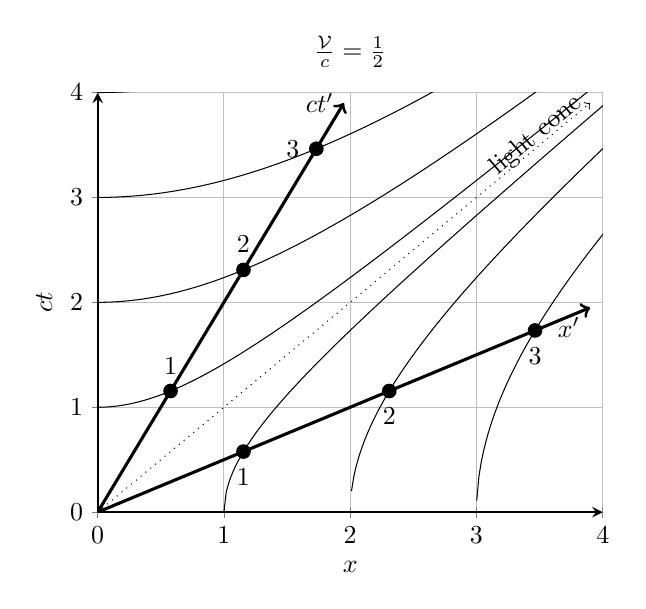
\begin{tikzpicture}[scale = .936] %1/2 invariant 
		\begin{axis}[
		axis lines = left,
		axis line style = thick,
		title = {$\frac{\mathcal{V}}{c} = \frac{1}{2}$},
		grid = both,
		xlabel = $x$,
		ylabel = {$ct$},
		xmin = 0, xmax = 4,
		ymin = 0, ymax = 4,
		]	
		
		\addplot [domain = 0:3.9, dotted, ->] 
		{x} 
		[allow upside down = true, yshift = 5 pt, sloped] node [pos = .89] {light cone};
		\addplot [very thick, domain = 0:3.9, ->]
		{x/2} 
		[sloped] node[below left] {$x'$};
		\addplot [very thick, domain = 0:1.95, ->] 
		{2*x} 
		[sloped] node[left] {$ct'$};
		\addplot [samples = 500, domain = 1:10] {sqrt(x^2-1)} ;
		\addplot [samples = 500, domain = 0:10] {sqrt(x^2+1)} ;
		\addplot [samples = 500, domain = 1:10] {sqrt(x^2-4)} ;
		\addplot [samples = 500, domain = 0:10] {sqrt(x^2+4)} ;
		\addplot [samples = 500, domain = 1:10] {sqrt(x^2-9)} ;
		\addplot [samples = 500, domain = 0:10] {sqrt(x^2+9)} ;
		\addplot [samples = 500, domain = 1:10] {sqrt(x^2-16)} ;
		\addplot [samples = 500, domain = 0:10] {sqrt(x^2+16)} ;
		\coordinate [label = {below:$1$}, circle, fill, inner sep = 2 pt] 
		(x1) at (axis cs:({sqrt(4/3)}, {.5*sqrt(4/3)});
		\coordinate [label = {below:$2$}, circle, fill, inner sep = 2 pt] 
		(x2) at (axis cs:({2*sqrt(4/3)}, {sqrt(4/3)});
		\coordinate [label = {below:$3$}, circle, fill, inner sep = 2 pt] 
		(x3) at (axis cs:({3*sqrt(4/3)}, {3/2*sqrt(4/3)});
		\coordinate [label = {above:$1$}, circle, fill, inner sep = 2 pt] 
		(t1) at (axis cs:({.5*sqrt(4/3)}, {sqrt(4/3)});
		\coordinate [label = {above:$2$}, circle, fill, inner sep = 2 pt] 
		(t2) at (axis cs:({1*sqrt(4/3)}, {2*sqrt(4/3)});
		\coordinate [label = {left:$3$}, circle, fill, inner sep = 2 pt] 
		(t3) at (axis cs:({3/2*sqrt(4/3)}, {3*sqrt(4/3)});		
		\end{axis}
		\end{tikzpicture}
		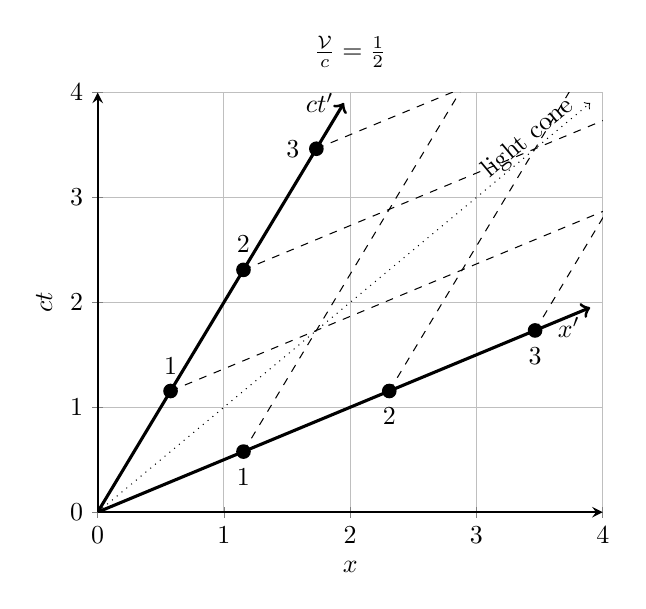
\begin{tikzpicture}[scale = .936] %1/2 world lines
		\begin{axis}[
		axis lines = left,
		axis line style = thick,
		title = {$\frac{\mathcal{V}}{c} = \frac{1}{2}$},
		grid = both,
		xlabel = $x$,
		ylabel = {$ct$},
		xmin = 0, xmax = 4,
		ymin = 0, ymax = 4,
		]	
		
		\addplot [domain = 0:3.9, dotted, ->] 
		{x} 
		[every node/.style = {yshift = 5 pt}, sloped] node[pos = .89] {light cone};
		\addplot [very thick, domain=0:3.9, ->]
		{x/2} 
		node[below left] {$x'$};
		\addplot [very thick, domain=0:1.95, ->] 
		{2*x} 
		node[left] {$ct'$};
		
		\addplot [dashed, domain = {sqrt(4/3)}:10] 
		{2*(x-sqrt(4/3))+.5*sqrt(4/3)};
		\coordinate [label = {below:$1$}, circle, fill, inner sep = 2 pt] 
		(x1) at (axis cs:({sqrt(4/3)}, {.5*sqrt(4/3)});
		
		\addplot [dashed, domain = {2*sqrt(4/3)}:10] 
		{2*(x-(2*sqrt(4/3)))+sqrt(4/3)};
		\coordinate [label = {below:$2$},circle, fill, inner sep = 2 pt] 
		(x2) at (axis cs:({2*sqrt(4/3)}, {sqrt(4/3)});
		
		\addplot [dashed, domain = {3*sqrt(4/3)}:10] 
		{2*(x-(3*sqrt(4/3)))+3/2*sqrt(4/3)};
		\coordinate [label = {below:$3$}, circle, fill, inner sep = 2 pt] 
		(x3) at (axis cs:({3*sqrt(4/3)}, {3/2*sqrt(4/3)});
		
		\addplot [dashed, domain = {.5*sqrt(4/3)}:10] 
		{.5*(x-(.5*sqrt(4/3)))+sqrt(4/3)};
		\coordinate [label = {above:$1$}, circle, fill, inner sep = 2 pt] 
		(t1) at (axis cs:({.5*sqrt(4/3)}, {sqrt(4/3)});
		
		\addplot [dashed, domain = {sqrt(4/3)}:10] 
		{.5*(x-(sqrt(4/3)))+2*sqrt(4/3)};
		\coordinate [label = {above:$2$}, circle, fill, inner sep = 2 pt] 
		(t2) at (axis cs:({1*sqrt(4/3)}, {2*sqrt(4/3)});
		
		\addplot [dashed, domain = {3/2*sqrt(4/3)}:10] 
		{.5*(x-(3/2*sqrt(4/3)))+3*sqrt(4/3)};
		\coordinate [label = {left:$3$}, circle, fill, inner sep = 2 pt] 
		(t3) at (axis cs:({3/2*sqrt(4/3)}, {3*sqrt(4/3)});
		\end{axis}
		\end{tikzpicture}\\ 
		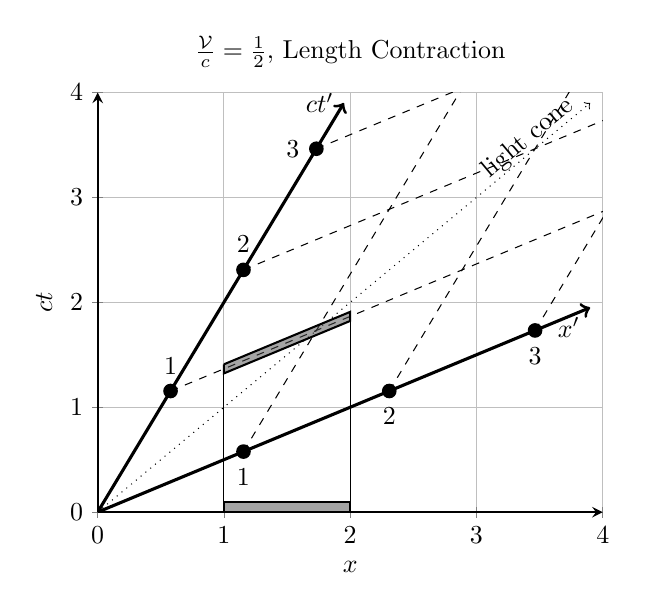
\begin{tikzpicture}[scale = .936] %1/2 length contraction
		\begin{axis}[
		axis lines = left,
		axis line style = thick,
		title = {$\frac{\mathcal{V}}{c} = \frac{1}{2}$, Length Contraction},
		grid = both,
		xlabel = $x$,
		ylabel = {$ct$},
		xmin = 0, xmax = 4,
		ymin = 0, ymax = 4,
		]	
		
		\addplot [domain = 0:3.9, dotted, ->] 
		{x} 
		[every node/.style = {yshift = 5pt}, sloped] node[pos = .89] {light cone};
		\addplot [very thick, domain = 0:3.9, ->] 
		{x/2} 
		node[below left] {$x'$};
		\addplot [very thick, domain = 0:1.95,->] 
		{2*x} 
		node[left] {$ct'$};
		
		\addplot [dashed, domain = {sqrt(4/3)}:10] 
		{2*(x-sqrt(4/3))+.5*sqrt(4/3)};
		\coordinate [label = {below:$1$}, circle, fill, inner sep = 2pt] 
		(x1) at (axis cs:({sqrt(4/3)}, {.5*sqrt(4/3)});
		
		\addplot [dashed, domain = {2*sqrt(4/3)}:10] 
		{2*(x-(2*sqrt(4/3)))+sqrt(4/3)};
		\coordinate [label = {below:$2$}, circle, fill, inner sep = 2pt] 
		(x2) at (axis cs:({2*sqrt(4/3)}, {sqrt(4/3)});
		
		\addplot [dashed, domain = {3*sqrt(4/3)}:10] 
		{2*(x-(3*sqrt(4/3)))+3/2*sqrt(4/3)};
		\coordinate [label = {below:$3$}, circle, fill, inner sep = 2pt] 
		(x3) at (axis cs:({3*sqrt(4/3)}, {3/2*sqrt(4/3)});
		
		\addplot [dashed, domain = {.5*sqrt(4/3)}:10] 
		{.5*(x-(.5*sqrt(4/3)))+sqrt(4/3)};
		\coordinate [label = {above=:$1$}, circle, fill, inner sep = 2pt] 
		(t1) at (axis cs:({.5*sqrt(4/3)}, {sqrt(4/3)});
		
		\addplot [dashed, domain = {sqrt(4/3)}:10] 
		{.5*(x-(sqrt(4/3)))+2*sqrt(4/3)};
		\coordinate [label = {above:$2$}, circle, fill, inner sep = 2pt] 
		(t2) at (axis cs:({1*sqrt(4/3)}, {2*sqrt(4/3)});
		
		\addplot [dashed, domain = {3/2*sqrt(4/3)}:10] 
		{.5*(x-(3/2*sqrt(4/3)))+3*sqrt(4/3)};
		\coordinate [label = {left:$3$}, circle, fill, inner sep = 2pt] 
		(t3) at (axis cs:({3/2*sqrt(4/3)}, {3*sqrt(4/3)});
		
		\draw[thick, color = black!200, fill = black!70, fill opacity = 0.5] 
		(axis cs:1,.1) rectangle (axis cs:2,0);
		
		
		%		\addplot [thick, color = black!200, mark = *, fill = black!70, fill opacity = 0.5] coordinates {(1,.1) (1,0) (2,0) (2,.1) (1,.1)};
		
		\addplot [mesh, black] 
		coordinates {
			(2,0) (2,{(.5*(2-(.5*sqrt(4/3)))+sqrt(4/3))-(sqrt(3)/40)})
		};			
		\addplot[mesh, black] 
		coordinates {
			(1,0) (1,{(.5*(1-(.5*sqrt(4/3)))+sqrt(4/3))-(sqrt(3)/40)})
		};
		
		%\draw[thick, color = black!200, fill = black!70, fill opacity = 0.5] (axis cs:1,{(.5*(1-(.5*sqrt(4/3)))+sqrt(4/3))+(sqrt(3)/40)}) line (axis cs:2,{(.5*(2-(.5*sqrt(4/3)))+sqrt(4/3))+(sqrt(3)/40)});
		\addplot [thick, color = black!200, fill = black!70, fill opacity = 0.5] 
		coordinates{
			(1,{(.5*(1-(.5*sqrt(4/3)))+sqrt(4/3))+(sqrt(3)/40)}) (1,{(.5*(1-(.5*sqrt(4/3)))+sqrt(4/3))-(sqrt(3)/40)}) (2,{(.5*(2-(.5*sqrt(4/3)))+sqrt(4/3))-(sqrt(3)/40)}) (2,{(.5*(2-(.5*sqrt(4/3)))+sqrt(4/3))+(sqrt(3)/40)}) (1,{(.5*(1-(.5*sqrt(4/3)))+sqrt(4/3))+(sqrt(3)/40)})
		};
		\end{axis}
		\end{tikzpicture}
		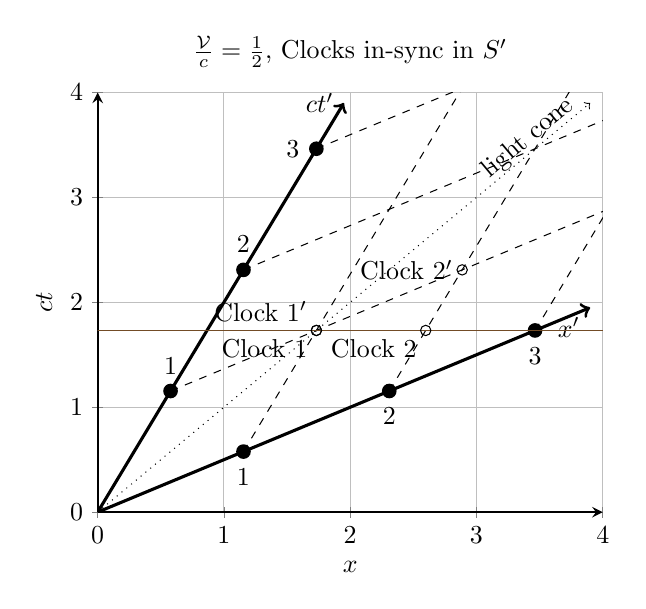
\begin{tikzpicture}[scale = .936] %1/2 time dilation
		\begin{axis}[
		axis lines = left,
		axis line style = thick,
		title = {$\frac{\mathcal{V}}{c}=\frac{1}{2}$, Clocks in-sync in $S'$},
		grid = both,
		xlabel = $x$,
		ylabel = {$ct$},
		xmin = 0, xmax = 4,
		ymin = 0, ymax = 4,
		]	
		
		
		\addplot [domain = 0:3.9, dotted, ->] 
		{x} 
		[every node/.style = {yshift = 5pt}, sloped] node[pos = .89] {light cone};
		\addplot [very thick, domain = 0:3.9, ->] 
		{x/2} 
		node[below left] {$x'$};
		\addplot [very thick, domain = 0:1.95, ->] 
		{2*x} 
		node[left] {$ct'$};
		
		\addplot [dashed, domain = {sqrt(4/3)}:10]
		{2*(x-sqrt(4/3))+.5*sqrt(4/3)};
		\coordinate [label = {below:$1$}, circle, fill, inner sep = 2pt] 
		(x1) at (axis cs:({sqrt(4/3)}, {.5*sqrt(4/3)});
		
		\addplot [dashed, domain = {2*sqrt(4/3)}:10] 
		{2*(x-(2*sqrt(4/3)))+sqrt(4/3)};
		\coordinate [label = {below:$2$}, circle, fill, inner sep = 2pt] 
		(x2) at (axis cs:({2*sqrt(4/3)}, {sqrt(4/3)});
		
		\addplot [dashed, domain = {3*sqrt(4/3)}:10] 
		{2*(x-(3*sqrt(4/3)))+3/2*sqrt(4/3)};
		\coordinate [label = {below:$3$}, circle, fill, inner sep = 2pt] 
		(x3) at (axis cs:({3*sqrt(4/3)}, {3/2*sqrt(4/3)});
		
		\addplot [dashed, domain = {.5*sqrt(4/3)}:10] 
		{.5*(x-(.5*sqrt(4/3)))+sqrt(4/3)};
		\coordinate [label = {above:$1$}, circle, fill, inner sep = 2pt] 
		(t1) at (axis cs:({.5*sqrt(4/3)}, {sqrt(4/3)});
		
		\addplot [dashed, domain = {sqrt(4/3)}:10] 
		{.5*(x-(sqrt(4/3)))+2*sqrt(4/3)};
		\coordinate [label = {above:$2$}, circle, fill, inner sep = 2pt] 
		(t2) at (axis cs:({1*sqrt(4/3)}, {2*sqrt(4/3)});
		
		\addplot [dashed, domain = {3/2*sqrt(4/3)}:10] 
		{.5*(x-(3/2*sqrt(4/3)))+3*sqrt(4/3)};
		\coordinate [label = {left:$3$}, circle, fill, inner sep = 2pt] 
		(t3) at (axis cs:({3/2*sqrt(4/3)}, {3*sqrt(4/3)});
		
		\addplot [mark = o] 
		coordinates {
			({3/2*sqrt(4/3)}, {3/2*sqrt(4/3)})} node[above left]{Clock $1'$
		};
		\addplot [mark = o] 
		coordinates {
			({3/2*sqrt(4/3)}, {3/2*sqrt(4/3)})
		} node[below left] {Clock $1$};
		\addplot [label = {left:Clock $2$}, mark = o] 
		coordinates {
			({5/2*sqrt(4/3)}, {2*sqrt(4/3)})
		} node[left] {Clock $2'$};
		\addplot coordinates {(-1,{3/2*sqrt(4/3)}) (10,{3/2*sqrt(4/3)})};
		\addplot [label = {left:Clock $2$}, mark = o] 
		coordinates {
			({9/4*sqrt(4/3)}, {3/2*sqrt(4/3)})
		} node[below left] {Clock $2$};
		\end{axis}
		\end{tikzpicture}\\
		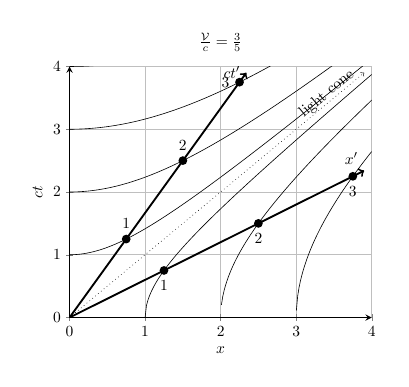
\begin{tikzpicture}[scale = .56] %3/5 invariant
		\begin{axis}[
		axis lines = left,
		axis line style = thick,
		title = {$\frac{\mathcal{V}}{c} = \frac{3}{5}$},
		grid = both,
		xlabel = $x$,
		ylabel = {$ct$},
		xmin = 0, xmax = 4,
		ymin = 0, ymax = 4,
		]	
		
		\addplot [domain = 0:3.9, dotted, ->] {x} [every node/.style = {yshift = 5pt}, sloped] node[pos = .89] {light cone};
		\addplot [very thick, domain = 0:3.9, ->] {3*x/5} node[above left] {$x'$};
		\addplot [very thick, domain = 0:2.34, ->] {5/3*x} node[left] {$ct'$};
		\addplot [samples = 500, domain = 1:10] {sqrt(x^2-1)} ;
		\addplot [samples = 500, domain = 0:10] {sqrt(x^2+1)} ;
		\addplot [samples = 500, domain = 1:10] {sqrt(x^2-4)} ;
		\addplot [samples = 500, domain = 0:10] {sqrt(x^2+4)} ;
		\addplot [samples = 500, domain = 1:10] {sqrt(x^2-9)} ;
		\addplot [samples = 500, domain = 0:10] {sqrt(x^2+9)} ;
		\addplot [samples = 500, domain = 1:10] {sqrt(x^2-16)} ;
		\addplot [samples = 500, domain = 0:10] {sqrt(x^2+16)} ;
		\coordinate [label = {below:$1$}, circle, fill, inner sep = 2pt] 
		(x1) at (axis cs:5/4,3/4);
		\coordinate [label = {below:$2$}, circle, fill, inner sep = 2pt] 
		(x2) at (axis cs:5/2,3/2);
		\coordinate [label = {below:$3$}, circle, fill, inner sep = 2pt] 
		(x3) at (axis cs:15/4,9/4);
		\coordinate [label = {above:$1$}, circle, fill,inner sep = 2pt] 
		(t1) at (axis cs:3/4,5/4);
		\coordinate [label = {above:$2$}, circle, fill, inner sep = 2pt] 
		(t2) at (axis cs:3/2,5/2);
		\coordinate [label = {left:$3$}, circle, fill, inner sep = 2pt] 
		(t3) at (axis cs:9/4,15/4);
		\end{axis}
		\end{tikzpicture}
		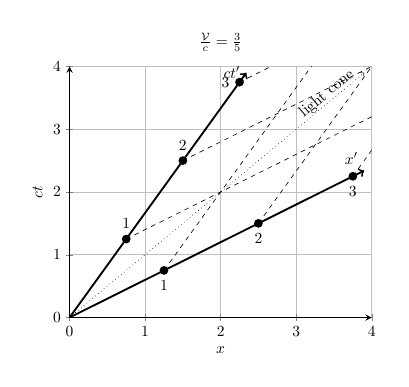
\begin{tikzpicture}[scale = .56] %3/5 world lines
		\begin{axis}[
		axis lines = left,
		axis line style=thick,
		title = {$\frac{\mathcal{V}}{c} = \frac{3}{5}$},
		grid = both,
		xlabel = $x$,
		ylabel = {$ct$},
		xmin = 0, xmax = 4,
		ymin = 0, ymax = 4,
		]	
		
		\addplot [domain = 0:3.9, dotted, ->] 
		{x} 
		[every node/.style = {yshift = 5pt}, sloped] node[pos = .89] {light cone};
		\addplot [very thick, domain = 0:3.9, ->] 
		{3*x/5} node[above left] {$x'$};
		\addplot [very thick, domain = 0:2.34, ->] 
		{5/3*x} node[left] {$ct'$};
		
		\addplot[dashed, domain = (5/4):10] 
		{(5/3)*(x-(5/4))+(3/4)};
		\coordinate [label = {below:$1$}, circle, fill, inner sep = 2pt] 
		(x1) at (axis cs:5/4,3/4);
		
		\addplot[dashed, domain = (5/2):10] 
		{(5/3)*(x-(5/2))+(3/2)};
		\coordinate [label = {below:$2$}, circle, fill, inner sep = 2pt] 
		(x2) at (axis cs:5/2,3/2);
		
		\addplot[dashed, domain = (15/4):10] 
		{(5/3)*(x-(15/4))+(9/4)};
		\coordinate [label = {below:$3$}, circle, fill, inner sep = 2pt] 
		(x3) at (axis cs:15/4,9/4);
		
		\addplot[dashed, domain = (3/4):10] 
		{(3/5)*(x-(3/4))+(5/4)};
		\coordinate [label = {above:$1$}, circle, fill, inner sep = 2pt] 
		(t1) at (axis cs:3/4,5/4);
		
		\addplot[dashed, domain = (3/2):10] 
		{(3/5)*(x-(3/2))+(5/2)};
		\coordinate [label = {above:$2$}, circle, fill, inner sep = 2pt] 
		(t2) at (axis cs:3/2,5/2);
		
		\addplot[dashed, domain = (9/4):10] 
		{(3/5)*(x-(9/4))+(15/4)};
		\coordinate [label = {left:$3$}, circle, fill, inner sep = 2pt] 
		(t3) at (axis cs:9/4,15/4);
		\end{axis}
		\end{tikzpicture}
		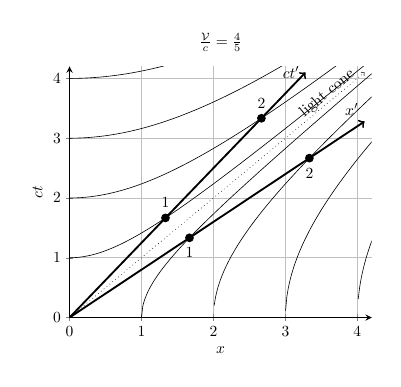
\begin{tikzpicture}[scale = .56] %4/5 invariant 
		\begin{axis}[
		axis lines = left,
		axis line style = thick,
		title = {$\frac{\mathcal{V}}{c} = \frac{4}{5}$},
		grid = both,
		xlabel = $x$,
		ylabel = {$ct$},
		xmin = 0, xmax = 4.2,
		ymin = 0, ymax = 4.2,
		]	
		
		\addplot [domain = 0:4.1, dotted, ->] 
		{x} 
		[every node/.style = {yshift = 5pt}, sloped] node[pos = .89] {light cone};
		\addplot [very thick, domain = 0:4.1, ->] 
		{4/5*x} node[above left] {$x'$};
		\addplot [very thick, domain = 0:82/25, ->] 
		{5/4*x} node[left] {$ct'$};
		\addplot [samples = 500, domain = 1:10] 
		{sqrt(x^2-1)};
		
		\addplot [samples = 500, domain = 0:10] 
		{sqrt(x^2+1)};
		
		\addplot [samples = 500, domain = 1:10] 
		{sqrt(x^2-4)};
		
		\addplot [samples = 500, domain = 0:10] 
		{sqrt(x^2+4)};
		
		\addplot [samples = 500, domain = 1:10] 
		{sqrt(x^2-9)};
		
		\addplot [samples = 500, domain = 0:10] 
		{sqrt(x^2+9)};
		
		\addplot [samples = 500, domain = 1:10] 
		{sqrt(x^2-16)};
		
		\addplot [samples = 500, domain = 0:10] 
		{sqrt(x^2+16)};
		
		\coordinate [label = {below:$1$}, circle, fill, inner sep = 2pt] 
		(x1) at (axis cs:5/3,4/3);
		\coordinate [label = {below:$2$}, circle, fill, inner sep = 2pt] 
		(x2) at (axis cs:2*5/3,8/3);
		\coordinate [label = {above:$1$}, circle, fill, inner sep = 2pt] 
		(t1) at (axis cs:4/3,5/3);
		\coordinate [label = {above:$2$}, circle, fill, inner sep = 2pt] 
		(t2) at (axis cs:8/3,10/3);
		\end{axis}
		\end{tikzpicture}
		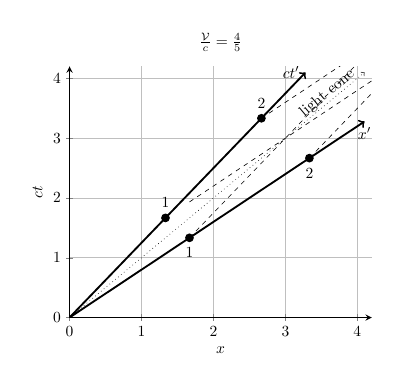
\begin{tikzpicture}[scale = .56] %4/5 world lines
		\begin{axis}[
		axis lines = left,
		axis line style = thick,
		title = {$\frac{\mathcal{V}}{c} = \frac{4}{5}$},
		grid = both,
		xlabel = $x$,
		ylabel = {$ct$},
		xmin = 0, xmax = 4.2,
		ymin = 0, ymax = 4.2,
		]	
		
		\addplot [domain = 0:4.1, dotted, ->] 
		{x} [every node/.style = {yshift = 5pt}, sloped] node[pos = .89] {light cone};
		\addplot [very thick, domain = 0:4.1, ->] 
		{4/5*x} node[below] {$x'$};
		\addplot [very thick, domain = 0:82/25, ->] 
		{5/4*x} node[left] {$ct'$};
		
		\addplot[dashed, domain = (5/3):10] 
		{(5/4)*(x-(5/3))+(4/3)};
		\coordinate [label = {below:$1$}, circle, fill, inner sep = 2pt] 
		(x1) at (axis cs:5/3,4/3);
		
		\addplot[dashed, domain = (10/3):10] 
		{(5/4)*(x-(10/3))+(8/3)};
		\coordinate [label = {below:$2$}, circle, fill, inner sep = 2pt] 
		(x2) at (axis cs:2*5/3,8/3);
		
		\addplot[dashed, domain = (5/3):10] 
		{(4/5)*(x-(4/3))+(5/3)};
		\coordinate [label = {above:$1$}, circle, fill, inner sep = 2pt] 
		(t1) at (axis cs:4/3,5/3);
		
		\addplot[dashed, domain = (8/3):10] 
		{(4/5)*(x-(8/3))+(10/3)};
		\coordinate [label = {above:$2$}, circle, fill, inner sep = 2pt] 
		(t2) at (axis cs:8/3,10/3);
		\end{axis}
		\end{tikzpicture}\\
	\end{center}

	\subsubsection*{Invariant:}
		\begin{dgroup*}\begin{dmath*}
		\left(x'\right)^2-\left(ct'\right)^2 \heq (x)^2-\left(ct\right)^2 = \pm a^2\end{dmath*}\begin{dmath*}
		\left(E'\right)^2 - \left(p'c\right)^2 \heq \left(E\right)^2 - \left(pc\right)^2 = m^2c^4
		\end{dmath*}\end{dgroup*}
	
	\subsubsection*{Einstein's Postulates:} \begin{enumerate}
		\item Absolute uniform motion cannot be detected.
		\item The velocity of light does not depend upon the velocity of its source.
	\end{enumerate}

	\subsubsection*{Momentum and Energy:} Where $v$ in $\frac{1}{\sqrt{1-\frac{v^2}{c^2}}}$ is given by $v=|\mathbf{v}|=\sqrt{v_x^2+v_y^2+v_z^2}$ the speed of the particle in that particular frame of reference and is different between two frames.
	\[
		\begin{array}{c|c}
		P_{\mu} = \left(P_0,P_x,P_y,P_z\right)	& P_0' = \frac{P_0-\frac{\mathcal{V} P_x}{c}}{\sqrt{1-\frac{\mathcal{V}^2}{c^2}}} \\ 
		P_{\mu} = \left(\frac{mc}{\sqrt{1-\frac{v^2}{c^2}}}, \frac{mv_x}{\sqrt{1-\frac{v^2}{c^2}}}, \frac{mv_y}{\sqrt{1-\frac{v^2}{c^2}}}, \frac{mv_z}{\sqrt{1-\frac{v^2}{c^2}}}\right)	&	P_x' = \frac{P_x-\frac{\mathcal{V} P_0}{c}}{\sqrt{1-\frac{\mathcal{V}^2}{c^2}}} \\ 
		\left(P_{\mu}\right)_{\text{initial}} = \left(P_{\mu}\right)_{\text{final}}	& \begin{array}{cc} P_y' = P_y & P_z' = P_z \end{array}
		\end{array}
	\]
	\[
	E_{\text{photon}} = hf = p_{\text{photon}}c
	\]
	\[	
		\begin{array}{c|c}
		E=\frac{1}{\sqrt{1-\frac{v^2}{c^2}}} mc^2	& E=mc^2+KE \\ 
		KE=\left(\frac{1}{\sqrt{1-\frac{v^2}{c^2}}}-1\right) mc^2	& E^2=m^2c^4+p^2c^2
		\end{array} 
	\]
	
	\subsubsection*{Relativistic Doppler Effect:}
	\[
	\begin{array}{c|c}
		\cos\left( \theta \right) = \frac{\cos\left( \theta' \right) + \frac{\mathcal{V}}{c}}{1+\frac{\mathcal{V}}{c}\cos\left( \theta' \right)}	&	\cos\left( \theta' \right) = \frac{\cos\left( \theta \right) - \frac{\mathcal{V}}{c}}{1 - \frac{\mathcal{V}}{c}\cos\left( \theta \right)}\\
		f_{\text{observed}} = f_{\text{emit}} \frac{\sqrt{1-\frac{\mathcal{V}^2}{c^2}}}{1-\frac{\mathcal{V}}{c}\cos\left( \theta \right)} = f_{\text{emit}} \sqrt{\frac{1 + \frac{\mathcal{V}}{c}}{1 - \frac{\mathcal{V}}{c}}}	&	\Delta\lambda = \frac{h}{m_e c} \left( 1 - \cos\left( \theta \right) \right) \longrightarrow\text{ ``Compton Scattering"}
	\end{array}
	\]
	
	
	\subsubsection*{Fixed Target Collisions:} If Particle $2$ is a stationary target and Particle $1$ strikes it in order to achieve energy $E'_T$ in the center of momentum frame then
%	\begin{dmath*}
%		{E_1 = \frac{{E^\prime_T}^2 - \left( m_1^2 + m_2^2 \right) c^4}{2 m_2 c^2}} \\
%		{\left( E_1 \right)_{\text{threshold}} = \frac{\left( \sum\limits_{\substack{\text{final} \\ \text{particles}}} {m c^2} \right)^2 - \left( m_1^2 + m_2^2 \right) c^4}{2 m_2 c^2}}
%	\end{dmath*}
	\begin{dgroup*}\begin{dmath*}
		E_1 = \frac{{E^\prime_T}^2 - \left( m_1^2 + m_2^2 \right) c^4}{2 m_2 c^2} \end{dmath*}\begin{dmath*}
		\left( E_1 \right)_{\text{threshold}} = \frac{\left( \sum\limits_{\substack{\text{final} \\ \text{particles}}} {m c^2} \right)^2 - \left( m_1^2 + m_2^2 \right) c^4}{2 m_2 c^2}
	\end{dmath*}\end{dgroup*}
	
	






\end{document}